\documentclass[10pt,a4paper]{article}
\usepackage[UTF8,fontset = windows]{ctex}
\setCJKmainfont[BoldFont=黑体,ItalicFont=楷体]{华文中宋}

\usepackage{pgfplots}
\pgfplotsset{compat=1.15}
\usepackage{amssymb,amsmath,amsfonts,amsthm,mathrsfs,dsfont,graphicx}
\usepackage{ifthen,indentfirst,enumerate,color,titletoc}
\usepackage{tikz}
\usepackage{multicol}
\usepackage{makecell}
\usepackage{longtable}
\usepackage{xcolor}
\usetikzlibrary{arrows,calc,intersections,patterns,decorations.pathreplacing,3d,angles}
\renewcommand{\baselinestretch}{1.65}
\newtheorem{defi}{定义~}
\newtheorem{eg}{例~}
\newtheorem{ex}{~}
\newtheorem{rem}{注~}
\newtheorem{thm}{定理~}
\newtheorem{coro}{推论~}
\newtheorem{axiom}{公理~}
\newtheorem{prop}{性质~}
\newcommand{\blank}[1]{\underline{\hbox to #1pt{}}}
\newcommand{\bracket}[1]{(\hbox to #1pt{})}
\newcommand{\onech}[4]{\par\begin{tabular}{p{.9\textwidth}}
A.~#1\\
B.~#2\\
C.~#3\\
D.~#4
\end{tabular}}
\newcommand{\twoch}[4]{\par\begin{tabular}{p{.46\textwidth}p{.46\textwidth}}
A.~#1& B.~#2\\
C.~#3& D.~#4
\end{tabular}}
\newcommand{\vartwoch}[4]{\par\begin{tabular}{p{.46\textwidth}p{.46\textwidth}}
(1)~#1& (2)~#2\\
(3)~#3& (4)~#4
\end{tabular}}
\newcommand{\fourch}[4]{\par\begin{tabular}{p{.23\textwidth}p{.23\textwidth}p{.23\textwidth}p{.23\textwidth}}
A.~#1 &B.~#2& C.~#3& D.~#4
\end{tabular}}
\newcommand{\varfourch}[4]{\par\begin{tabular}{p{.23\textwidth}p{.23\textwidth}p{.23\textwidth}p{.23\textwidth}}
(1)~#1 &(2)~#2& (3)~#3& (4)~#4
\end{tabular}}

\begin{document}

如图, 正方形$OABC$的边长为$a$($a>1$), 函数$y=3x^2$交$AB$于点$Q$, 函数$y=x^{-\frac 12}$与$BC$交于点$P$, 当$|AQ|+|CP|$最小时, $a$的值为\blank{50}.
\begin{center}
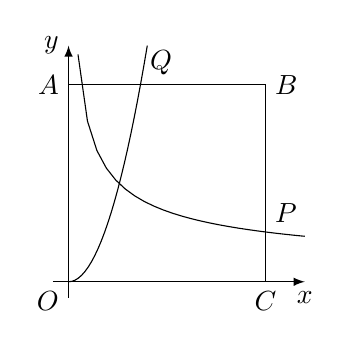
\begin{tikzpicture}[>=latex]
\draw [->] (-0.2,0) -- (3,0) node [below] {$x$};
\draw [->] (0,-0.2) -- (0,3) node [left] {$y$};
\draw (0,0) node [below left] {$O$};
\draw (2.5,0) node [below] {$C$} coordinate (C);
\draw (2.5,2.5) node [right] {$B$} coordinate (B);
\draw (0,2.5) node [left] {$A$} coordinate (A);
\draw [domain = 0:1] plot (\x,{3*\x*\x});
\draw [domain = 0.12:3] plot (\x,{pow(\x,-1/2)});
\draw (C) -- (B) -- (A);
\draw ({sqrt(2.5/3)},2.5) node [above right] {$Q$};
\draw (2.5,{pow(2.5,-1/2)}) node [above right] {$P$};
\end{tikzpicture}
\end{center}

已知$a<0<b<|a|$, 且集合$A=\{x|a<x\le b, \ x\in \mathbf{R}\}$, $B=\{x|-b<x\le -a, \ x\in \mathbf{R}\}$, 则$A\cap B=$\blank{50}, $A\cup B=$\blank{50}.

%\input{"../题库0.2/相似题目_待处理01.txt"}

%\begin{enumerate}[1.]
%\input{"g:/Temp/vault_test/排列组合.tex"}
%\end{enumerate}

\end{document}